%%%%%%%%%%%%%%%%%%%%%%%%%%%%%%%%%%%%%%%%%%%%%%%%%%%%%%%%%%%%%%%%%%%%%%%%%%%%%%%%%%
\begin{frame}[fragile]\frametitle{}
\begin{center}
{\Large Semantics}
\end{center}
\end{frame}


%%%%%%%%%%%%%%%%%%%%%%%%%%%%%%%%%%%%%%%%%%%%%%%%%%%%%%%%%%%%%%%%%%%%%%%%%%%%%%%%%%
\begin{frame}[fragile]\frametitle{What is Semantics?}
  \begin{itemize}
    \item Semantics is the study of meaning in language and symbols.
    \item In the context of Knowledge Graphs, semantics provides context and understanding to data.
    \item It helps bridge the gap between human understanding and machine processing.
  \end{itemize}

\begin{center}
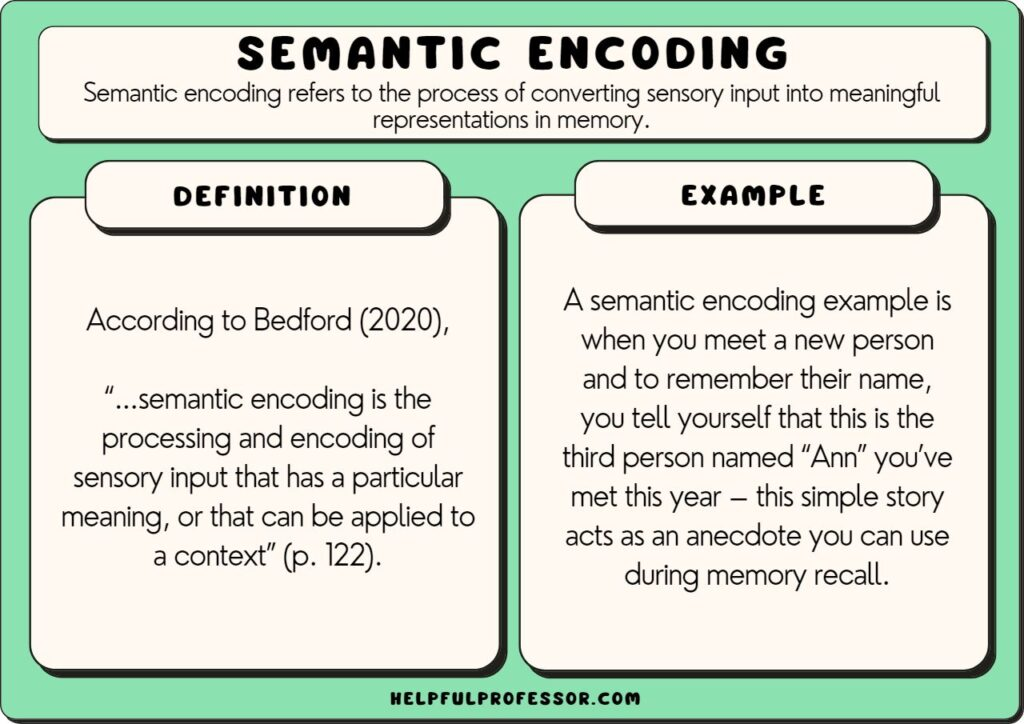
\includegraphics[width=0.6\linewidth,keepaspectratio]{semantics}

{\tiny (Ref: Semantic Encoding: 10 Examples and Definition (2023))}
\end{center}	
  
\end{frame}  


%%%%%%%%%%%%%%%%%%%%%%%%%%%%%%%%%%%%%%%%%%%%%%%%%%%%%%%%%%%%%%%%%%%%%%%%%%%%%%%%%%
\begin{frame}[fragile]\frametitle{The Power of Knowledge Graphs}
  \begin{itemize}
    \item Knowledge Graphs are powerful data structures representing information as nodes and edges.
    \item They capture complex relationships and connections between entities.
    \item Semantics enrich Knowledge Graphs by attributing meaning to these entities and relationships.
    \item This deepens data understanding and enables advanced analysis and decision-making.
  \end{itemize}
  
\begin{center}
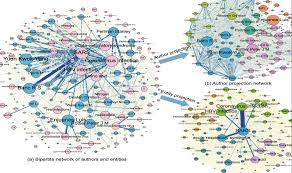
\includegraphics[width=0.6\linewidth,keepaspectratio]{kg22}

{\tiny (Ref: PubMed Knowledge Graph – AI Health Lab)}

\end{center}	  
\end{frame}

%%%%%%%%%%%%%%%%%%%%%%%%%%%%%%%%%%%%%%%%%%%%%%%%%%%%%%%%%%%%%%%%%%%%%%%%%%%%%%%%%%
\begin{frame}[fragile]\frametitle{Context Matters}
  \begin{itemize}
    \item In Knowledge Graphs, semantics add context to data.
    \item Consider a person named "Suresh" - semantics help distinguish if it's "Suresh Sharma" or "Suresh Varma."
    \item By understanding context, insurers gain insights into customer preferences, risks, and more.
    \item Semantics enable personalized customer experiences and targeted insurance products.
  \end{itemize}
\end{frame}

%%%%%%%%%%%%%%%%%%%%%%%%%%%%%%%%%%%%%%%%%%%%%%%%%%%%%%%%%%%%%%%%%%%%%%%%%%%%%%%%%%
\begin{frame}[fragile]\frametitle{Semantic Triplets}
  \begin{itemize}
    \item Knowledge Graphs use semantic triplets: Subject - Predicate - Object.
    \item Subject: The entity about which information is stored.
    \item Predicate: The relationship between the subject and the object.
    \item Object: The value or entity related to the subject.
    \item For example, (Ramesh, hasOccupation, Software Engineer) is a semantic triplet.
  \end{itemize}
  
\begin{center}
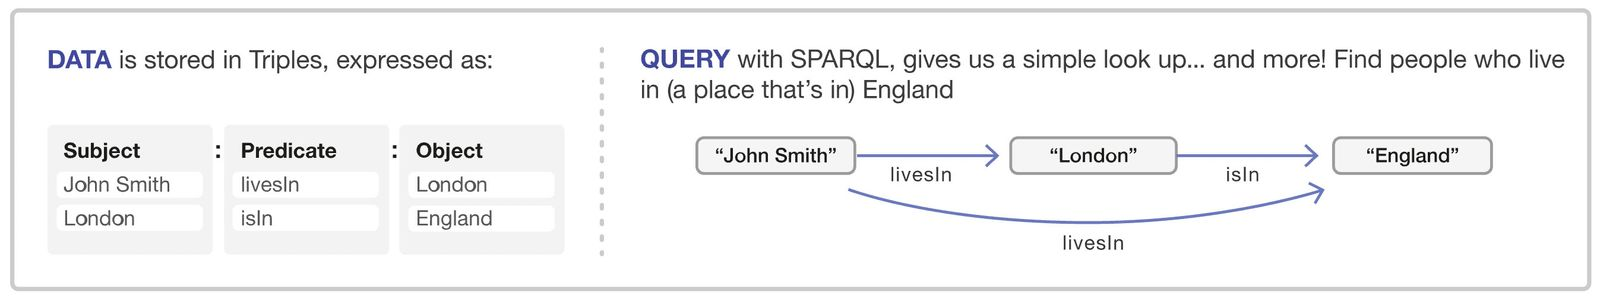
\includegraphics[width=\linewidth,keepaspectratio]{semantic1}

{\tiny (Ref: Semantic Triple - SEO North)}

\end{center}  
\end{frame}

%%%%%%%%%%%%%%%%%%%%%%%%%%%%%%%%%%%%%%%%%%%%%%%%%%%%%%%%%%%%%%%%%%%%%%%%%%%%%%%%%%
\begin{frame}[fragile]\frametitle{Unleashing the Potential}

\begin{columns}
    \begin{column}[T]{0.6\linewidth}
		  \begin{itemize}
			\item By leveraging semantics, insurers unlock hidden insights within their data.
			\item Semantics facilitate data integration, enriching the Knowledge Graph with diverse sources.
			\item Complex queries become manageable, leading to faster, data-driven decisions.
			\item The insurance industry can provide innovative products tailored to specific customer needs.
		  \end{itemize}
    \end{column}
    \begin{column}[T]{0.4\linewidth}  
		\begin{center}
		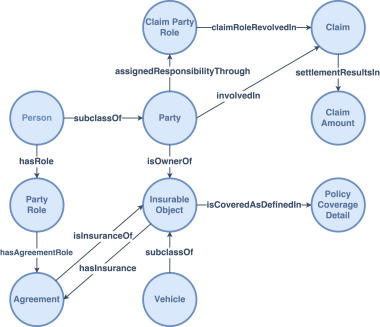
\includegraphics[width=\linewidth,keepaspectratio]{kg23}

		{\tiny (Ref: A standards-based ontology and support for Big Data Analytics in the insurance)}
		\end{center}    
    \end{column}
  \end{columns}
\end{frame}

%%%%%%%%%%%%%%%%%%%%%%%%%%%%%%%%%%%%%%%%%%%%%%%%%%%%%%%%%%%%%%%%%%%%%%%%%%%%%%%%%%
\begin{frame}[fragile]\frametitle{Real-world Applications}
  \begin{itemize}
    \item Customer Profiling: Semantics enable comprehensive customer 360 views for personalized interactions.
    \item Risk Assessment: Understand risk factors by connecting relevant data points.
    \item Fraud Detection: Uncover hidden patterns and detect fraudulent activities.
    \item Claims Management: Improve efficiency with insights from interconnected data.
  \end{itemize}
\end{frame}

%%%%%%%%%%%%%%%%%%%%%%%%%%%%%%%%%%%%%%%%%%%%%%%%%%%%%%%%%%%%%%%%%%%%%%%%%%%%%%%%%%
\begin{frame}[fragile]\frametitle{Challenges \& Considerations}
  \begin{itemize}
    \item Data Quality: Garbage in, garbage out - accurate data is crucial for meaningful semantics.
    \item Ontology Design: Thoughtful ontology creation ensures effective representation of concepts and relationships.
    \item Scalability: As data grows, the Knowledge Graph must handle increased complexity efficiently.
    \item Privacy and Security: Safeguarding sensitive data is paramount in the insurance industry.
  \end{itemize}
\end{frame}

%%%%%%%%%%%%%%%%%%%%%%%%%%%%%%%%%%%%%%%%%%%%%%%%%%%%%%%%%%%%%%%%%%%%%%%%%%%%%%%%%%
\begin{frame}[fragile]\frametitle{Embracing the Future}
  \begin{itemize}
    \item The adoption of Knowledge Graphs with semantics is transforming the insurance industry.
    \item Insurers embracing this technology gain a competitive advantage and drive innovation.
    \item Stay ahead of the curve by investing in semantic technologies and data-driven approaches.
    \item Embrace the potential of semantics to deliver better customer experiences and operational efficiency.
  \end{itemize}
\end{frame}

%%%%%%%%%%%%%%%%%%%%%%%%%%%%%%%%%%%%%%%%%%%%%%%%%%%%%%%%%%%%%%%%%%%%%%%%%%%%%%%%%%
\begin{frame}[fragile]\frametitle{Knowledge Graphs in Action}
  \begin{itemize}
    \item Let's take a look at a practical application of Knowledge Graph Semantics in insurance.
    \item Explore how semantics enhance data understanding and drive meaningful insights.
    \item Witness firsthand how insurers are benefiting from this transformative technology.
  \end{itemize}
\end{frame}

%%%%%%%%%%%%%%%%%%%%%%%%%%%%%%%%%%%%%%%%%%%%%%%%%%%%%%%%%%%%%%%%%%%%%%%%%%%%%%%%%%
\begin{frame}[fragile]\frametitle{}
\begin{center}
{\Large Taxonomy}
\end{center}
\end{frame}


%%%%%%%%%%%%%%%%%%%%%%%%%%%%%%%%%%%%%%%%%%%%%%%%%%%%%%%%%%%%%%%%%%%%%%%%%%%%%%%%%%
\begin{frame}[fragile]
\frametitle{Taxonomy in Semantics}

\begin{columns}
    \begin{column}[T]{0.6\linewidth}
		\begin{itemize}
		\item Taxonomy is a hierarchical classification system that organizes entities based on their characteristics and relationships.
		\item In Knowledge Graphs, taxonomy helps define the structure and categorization of information, improving data consistency and accuracy.
		\item By using taxonomy, insurers can create a clear and logical framework for their knowledge base, simplifying data integration and analysis.
		\end{itemize}

    \end{column}
    \begin{column}[T]{0.4\linewidth}  
		\begin{center}
		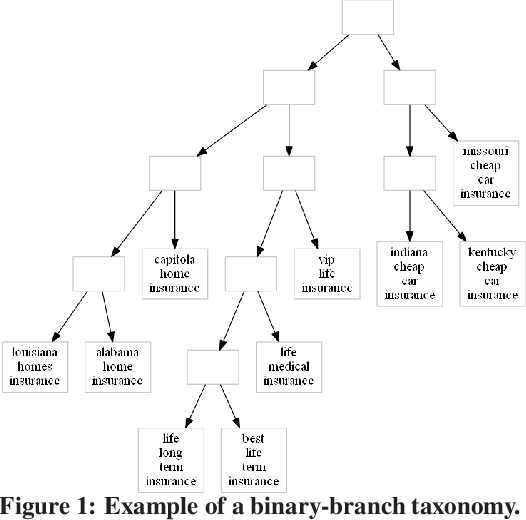
\includegraphics[width=\linewidth,keepaspectratio]{kg24}

		{\tiny (Ref: Automatic taxonomy construction from keywords)}
		\end{center}    
    \end{column}
  \end{columns}

\end{frame}

%%%%%%%%%%%%%%%%%%%%%%%%%%%%%%%%%%%%%%%%%%%%%%%%%%%%%%%%%%%%%%%%%%%%%%%%%%%%%%%%%%
\begin{frame}[fragile]
\frametitle{Advantages of Taxonomy in Insurance}
\begin{itemize}
\item Seamless Data Integration: Taxonomy ensures data from various sources can be integrated and understood uniformly.
\item Faster Decision Making: Well-defined taxonomy enables quicker access to relevant information, leading to faster and more accurate decisions.
\item Improved Customer Experience: Enhanced organization and retrieval of data enable a better understanding of customer needs, leading to personalized services.
\end{itemize}
\end{frame}

%%%%%%%%%%%%%%%%%%%%%%%%%%%%%%%%%%%%%%%%%%%%%%%%%%%%%%%%%%%%%%%%%%%%%%%%%%%%%%%%%%
\begin{frame}[fragile]
\frametitle{Building a Taxonomy}
\begin{itemize}
\item Identify Key Entities: Start by identifying crucial entities in your insurance domain, such as policies, claims, beneficiaries, etc.
\item Define Relationships: Establish meaningful relationships between entities, like 'owns,' 'insured by,' 'dependent on,' etc.
\item Hierarchical Structure: Organize entities into a hierarchical structure to create a clear taxonomy.
\item Flexibility and Scalability: Keep the taxonomy flexible to adapt to evolving needs and ensure it can scale with growing data.
\end{itemize}
\end{frame}

%%%%%%%%%%%%%%%%%%%%%%%%%%%%%%%%%%%%%%%%%%%%%%%%%%%%%%%%%%%%%%%%%%%%%%%%%%%%%%%%%%
\begin{frame}[fragile]
\frametitle{Example of Taxonomy}
\begin{figure}[h]
\centering
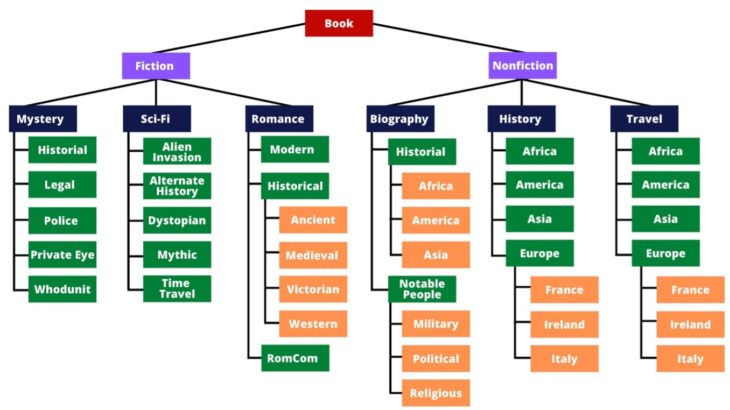
\includegraphics[width=0.8\textwidth]{taxonomy_example}
\caption{Example Taxonomy for Books}
\end{figure}

There are no absolute right and wrong with taxonomies, just degrees of appropriateness. The most important question to ask when creating a taxonomy is, “does this hierarchical grouping meet my needs?”
\end{frame}

%%%%%%%%%%%%%%%%%%%%%%%%%%%%%%%%%%%%%%%%%%%%%%%%%%%%%%%%%%%%%%%%%%%%%%%%%%%%%%%%%%
\begin{frame}[fragile]
\frametitle{Knowledge Graph and Taxonomy Integration}
\begin{itemize}
\item A Knowledge Graph can leverage the defined taxonomy to enhance its structure and relationships.
\item Taxonomy acts as a backbone for organizing information within the Knowledge Graph, making it more intuitive to navigate.
\item Queries and Insights: Taxonomy-driven Knowledge Graphs enable more precise queries and provide deeper insights into relationships between entities.
\end{itemize}
\end{frame}

%%%%%%%%%%%%%%%%%%%%%%%%%%%%%%%%%%%%%%%%%%%%%%%%%%%%%%%%%%%%%%%%%%%%%%%%%%%%%%%%%%
\begin{frame}[fragile]
\frametitle{Use Cases in the Insurance Industry}
\begin{itemize}
\item Claims Processing: Streamlining claims processing through efficient taxonomy-based data retrieval.
\item Customer Service: Enhancing customer service by understanding customer profiles and offering tailored insurance products.
\item Fraud Detection: Improving fraud detection by identifying suspicious patterns and connections between entities.
\item Risk Assessment: Facilitating risk assessment by analyzing correlations between policyholders and claims history.
\end{itemize}
\end{frame}

%%%%%%%%%%%%%%%%%%%%%%%%%%%%%%%%%%%%%%%%%%%%%%%%%%%%%%%%%%%%%%%%%%%%%%%%%%%%%%%%%%
\begin{frame}[fragile]
\frametitle{Conclusion}
\begin{itemize}
\item Taxonomy in Semantics plays a pivotal role in shaping powerful Knowledge Graphs for the insurance industry.
\item It provides a structured and standardized approach to organizing information, enabling better decision-making and customer experiences.
\item Embracing taxonomy-driven Knowledge Graphs empowers insurers to stay competitive and agile in an ever-evolving industry landscape.
\end{itemize}
\end{frame}


%%%%%%%%%%%%%%%%%%%%%%%%%%%%%%%%%%%%%%%%%%%%%%%%%%%%%%%%%%%%%%%%%%%%%%%%%%%%%%%%%%
\begin{frame}[fragile]\frametitle{}
\begin{center}
{\Large Ontology }
\end{center}
\end{frame}

%%%%%%%%%%%%%%%%%%%%%%%%%%%%%%%%%%%%%%%%%%%%%%%%%%%%%%%%%%%%%%%%%%%%%%%%%%%%%%%%%%
\begin{frame}[fragile]
\frametitle{Overview}
\begin{itemize}
\item Ontology: onto (existence, real) + logia (study) : most essential existence representation
\item According to Wikipedia, an ontology “encompasses a representation, formal naming, and definition of the categories, properties, and relations between the concepts, data, and entities that substantiate one, many, or all domains of discourse.”
\item In other words, ontologies allow us to organize the jargon of a subject area into a controlled vocabulary, thereby decreasing complexity and confusion. 
\item Without ontologies, you have no frame of reference, and understanding is lost.
\item For example, an ontology will allow one to associate the Book taxonomy with the Customer taxonomy via relationships.
\item An ontology is more challenging to create than a taxonomy because it needs to capture the interrelationships between business objects/concepts by encapsulating the language and terminology of the business area you are modeling.
\item Ontologies take taxonomy a step-further, by providing added layers to that relationship that and take it outside of just the product domain to other domains such as customer data and digital assets.   
\end{itemize}
\end{frame}

%%%%%%%%%%%%%%%%%%%%%%%%%%%%%%%%%%%%%%%%%%%%%%%%%%%%%%%%%%%%%%%%%%%%%%%%%%%%%%%%%%
\begin{frame}[fragile]
\frametitle{Understanding Ontology}
\begin{itemize}
\item Ontology is the backbone of Knowledge Graphs, providing a formal, shared understanding of the domain's concepts and relationships.
\item It defines the vocabulary and rules for representing and reasoning about the data, ensuring consistency and accuracy.
\item In the insurance industry, ontology can capture complex relationships between insurance products, coverage options, and risk factors.
\end{itemize}
\end{frame}

%%%%%%%%%%%%%%%%%%%%%%%%%%%%%%%%%%%%%%%%%%%%%%%%%%%%%%%%%%%%%%%%%%%%%%%%%%%%%%%%%%
\begin{frame}[fragile]
\frametitle{Advantages of Ontology in Insurance}

\begin{columns}
    \begin{column}[T]{0.6\linewidth}
		\begin{itemize}
		\item Enhanced Data Integration: Ontology allows for seamless integration of diverse data sources, leading to a more comprehensive view of customers and policies.
		\item Improved Search and Navigation: Ontology-driven Knowledge Graphs enable intuitive search and navigation, making it easier to find relevant information.
		\item Better Decision Making: With a formal understanding of concepts and relationships, insurers can make more informed and data-driven decisions.
		\end{itemize}

    \end{column}
    \begin{column}[T]{0.4\linewidth}  
		\begin{center}
		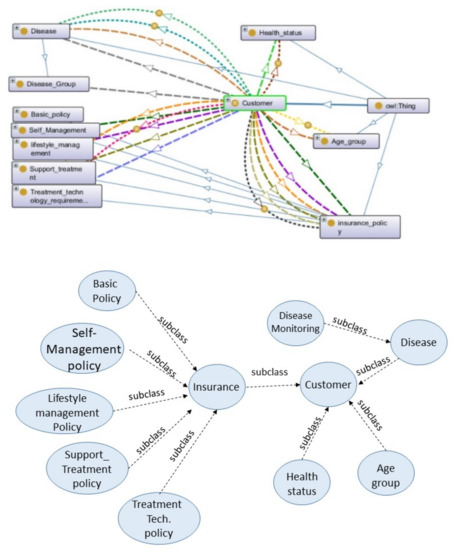
\includegraphics[width=\linewidth,keepaspectratio]{kg25}

		{\tiny (Ref: A-SHIP: Ontology-Based Adaptive Sustainable Healthcare Insurance Policy)}
		\end{center}    
    \end{column}
  \end{columns}
\end{frame}

%%%%%%%%%%%%%%%%%%%%%%%%%%%%%%%%%%%%%%%%%%%%%%%%%%%%%%%%%%%%%%%%%%%%%%%%%%%%%%%%%%
\begin{frame}[fragile]
\frametitle{Key Components of an Ontology}
\begin{enumerate}
\item \textbf{Classes:}
\begin{itemize}
\item Classes represent concepts or categories of objects in the domain.
\item In insurance, classes could include "Policy," "Customer," "Claim," etc.
\end{itemize}

\item \textbf{Properties:}
\begin{itemize}
\item Properties define relationships between classes or properties and classes.
\item Examples include "hasPolicy," "isInsuredBy," "belongsTo," etc.
\end{itemize}

\item \textbf{Individuals:}
\begin{itemize}
\item Individuals are instances of classes, representing specific objects or entities in the domain.
\item For instance, a specific insurance policy, customer, or claim can be considered individuals.
\end{itemize}

\item \textbf{Axioms and Constraints:}
\begin{itemize}
\item Axioms and constraints specify rules and logical relationships between classes and properties.
\item They enable reasoning and inferencing in the Knowledge Graph.
\end{itemize}

\item \textbf{Hierarchy and Inheritance:}
\begin{itemize}
\item Ontologies can have hierarchies, with classes inheriting characteristics from parent classes.
\item For example, a "Health Insurance Policy" inherits properties from the "Insurance Policy" class.
\end{itemize}
\end{enumerate}
\end{frame}


%%%%%%%%%%%%%%%%%%%%%%%%%%%%%%%%%%%%%%%%%%%%%%%%%%%%%%%%%%%%%%%%%%%%%%%%%%%%%%%%%%
\begin{frame}[fragile]
\frametitle{Building an Ontology}
\begin{itemize}
\item Identify Key Concepts: Start by identifying the fundamental concepts in the insurance domain, such as policies, claims, beneficiaries, etc.
\item Define Relationships: Establish relationships like 'has policy,' 'covered by,' 'owns,' etc., to represent connections between concepts.
\item Formalize Vocabulary: Create a formal vocabulary that standardizes the representation of concepts and their attributes.
\item Iterative Process: Ontology development is iterative and may evolve as domain knowledge deepens and business requirements change.
\end{itemize}
\end{frame}

%%%%%%%%%%%%%%%%%%%%%%%%%%%%%%%%%%%%%%%%%%%%%%%%%%%%%%%%%%%%%%%%%%%%%%%%%%%%%%%%%%
\begin{frame}[fragile]
\frametitle{Example of Ontology}
\begin{figure}[h]
\centering
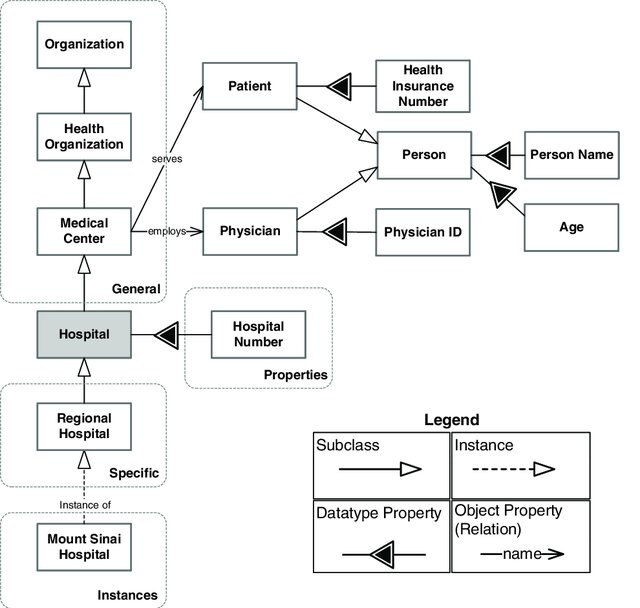
\includegraphics[width=0.5\textwidth]{ontology_example}
\caption{Example Ontology}

{\tiny (Ref: A semantic approach to approximate service retrieval)}
\end{figure}
\end{frame}

%%%%%%%%%%%%%%%%%%%%%%%%%%%%%%%%%%%%%%%%%%%%%%%%%%%%%%%%%%%%%%%%%%%%%%%%%%%%%%%%%%
\begin{frame}[fragile]
\frametitle{Knowledge Graph and Ontology Integration}
\begin{itemize}
\item Ontology forms the foundation of a Knowledge Graph, providing structure and meaning to the data.
\item It ensures that data is organized in a way that aligns with the domain's concepts and relationships.
\item Integration allows for powerful querying, reasoning, and inferencing within the Knowledge Graph.
\end{itemize}
\end{frame}

%%%%%%%%%%%%%%%%%%%%%%%%%%%%%%%%%%%%%%%%%%%%%%%%%%%%%%%%%%%%%%%%%%%%%%%%%%%%%%%%%%
\begin{frame}[fragile]
\frametitle{Use Cases in the Insurance Industry}
\begin{itemize}
\item Customer Profiling: Creating comprehensive customer profiles based on their policies, claims, and interactions.
\item Risk Assessment: Analyzing data from various sources to assess risks associated with insured entities.
\item Personalized Recommendations: Offering tailored insurance products and coverage options based on individual customer needs.
\item Fraud Detection: Identifying potential fraudulent activities by detecting anomalies in data patterns.
\end{itemize}
\end{frame}

%%%%%%%%%%%%%%%%%%%%%%%%%%%%%%%%%%%%%%%%%%%%%%%%%%%%%%%%%%%%%%%%%%%%%%%%%%%%%%%%%%
\begin{frame}[fragile]
\frametitle{Conclusion}
\begin{itemize}
\item Ontology in Semantics is a fundamental component of Knowledge Graphs that empowers the insurance industry with data-driven insights.
\item It enables a formal understanding of complex relationships between insurance concepts, leading to improved decision-making and customer experiences.
\item Embracing ontology-driven Knowledge Graphs positions insurers to thrive in an increasingly competitive and data-centric landscape.
\end{itemize}
\end{frame}


%%%%%%%%%%%%%%%%%%%%%%%%%%%%%%%%%%%%%%%%%%%%%%%%%%%%%%%%%%%%%%%%%%%%%%%%%%%%%%%%%%
\begin{frame}[fragile]\frametitle{}
\begin{center}
{\Large Key Differences between Taxonomy, Ontology, and Knowledge Graphs }
\end{center}
\end{frame}


%%%%%%%%%%%%%%%%%%%%%%%%%%%%%%%%%%%%%%%%%%%%%%%%%%%%%%%%%%%%%%%%%%%%%%%%%%%%%%%%%%
\begin{frame}[fragile]
\frametitle{Taxonomy}

\begin{itemize}
\item Focuses on hierarchical classification of entities based on their shared characteristics.
\item Typically employs a tree-like structure with parent-child relationships.
\item Provides a simple and intuitive way to categorize and organize data.
\item Primarily used for browsing and basic information retrieval.
\end{itemize}
\end{frame}

%%%%%%%%%%%%%%%%%%%%%%%%%%%%%%%%%%%%%%%%%%%%%%%%%%%%%%%%%%%%%%%%%%%%%%%%%%%%%%%%%%
\begin{frame}[fragile]
\frametitle{Ontology}
\begin{itemize}
\item Defines a formal, shared vocabulary that represents concepts and their relationships within a specific domain.
\item Captures the meaning and semantics of the data, enabling reasoning and inferencing.
\item Utilized for more advanced data integration, reasoning, and complex information retrieval.
\item Acts as the backbone of a Knowledge Graph, providing a foundation for structuring and understanding data.
\end{itemize}
\end{frame}


%%%%%%%%%%%%%%%%%%%%%%%%%%%%%%%%%%%%%%%%%%%%%%%%%%%%%%%%%%%%%%%%%%%%%%%%%%%%%%%%%%
\begin{frame}[fragile]
\frametitle{Knowledge Graphs}
\begin{itemize}
\item Represent interconnected data as entities and their relationships, forming a graph structure.
\item Utilizes ontology to define the schema and provide a formal representation of domain knowledge.
\item Enables sophisticated queries, data analysis, and inference through graph-based algorithms.
\item Offers a holistic view of data, empowering data-driven insights and decision-making in the insurance industry.
\end{itemize}
\end{frame}

%%%%%%%%%%%%%%%%%%%%%%%%%%%%%%%%%%%%%%%%%%%%%%%%%%%%%%%%%%%%%%%%%%%%%%%%%%%%%%%%%%
\begin{frame}[fragile]\frametitle{}
\begin{center}
{\Large Semantics Standards: RDF, RDFS, OWL }
\end{center}
\end{frame}

%%%%%%%%%%%%%%%%%%%%%%%%%%%%%%%%%%%%%%%%%%%%%%%%%%%%%%%%%%%%%%%%%%%%%%%%%%%%%%%%%%
\begin{frame}[fragile]
\frametitle{Understanding RDF, RDFS, and OWL}
\begin{itemize}
\item RDF (Resource Description Framework), RDFS (RDF Schema), and OWL (Web Ontology Language) are fundamental semantic web standards.
\item These standards play a crucial role in knowledge representation and reasoning within Knowledge Graphs.
\item In the insurance industry, these standards enable the development of rich and structured data models to drive better insights and decision-making.
\end{itemize}
\end{frame}

%%%%%%%%%%%%%%%%%%%%%%%%%%%%%%%%%%%%%%%%%%%%%%%%%%%%%%%%%%%%%%%%%%%%%%%%%%%%%%%%%%
\begin{frame}[fragile]
\frametitle{Key Features and Use Cases}
\begin{itemize}
\item \textbf{RDF (Resource Description Framework):}
\begin{itemize}
\item Defines a simple model to describe resources and their relationships using subject-predicate-object triples.
\item Use Cases: Capturing and linking data about policies, claims, customers, and other entities in the insurance domain.
\end{itemize}

\item \textbf{RDFS (RDF Schema):}
\begin{itemize}
\item Adds schema, resources, class, datatype, etc
\item Provides a basic vocabulary for creating hierarchies and defining classes and properties.
\item Use Cases: Specifying insurance-related concepts, properties, and their relationships in a structured manner.
\end{itemize}

\item \textbf{OWL (Web Ontology Language):}
\begin{itemize}
\item Offers more expressive power for defining classes, properties, and relationships, enabling advanced reasoning and inferencing.
\item Use Cases: Building complex insurance domain ontologies to support intelligent querying, fraud detection, and risk assessment.
\end{itemize}
\end{itemize}
\end{frame}


%%%%%%%%%%%%%%%%%%%%%%%%%%%%%%%%%%%%%%%%%%%%%%%%%%%%%%%%%%%%%%%%%%%%%%%%%%%%%%%%%%
\begin{frame}[fragile]
\frametitle{Key Features and Applications of RDF}
\begin{itemize}
\item \textbf{Subject-Predicate-Object Triples:}
\begin{itemize}
\item RDF represents information as triples, consisting of subject-predicate-object, forming a relationship statement.
\item Example: "Policy A (subject) hasCoverage (predicate) Auto (object)."
\end{itemize}

\item \textbf{Resource Identification:}
\begin{itemize}
\item Each resource in RDF is assigned a unique URI, enabling easy identification and linking of related data.
\item Example: A URI can uniquely represent a policy, a customer, or a claim in the insurance domain.
\end{itemize}

\item \textbf{Linked Data:}
\begin{itemize}
\item RDF facilitates the creation of Linked Data by connecting resources across the web, forming a vast knowledge network.
\item Use Cases: Cross-referencing insurance policies from different providers or analyzing industry trends by linking relevant data sources.
\end{itemize}

\item \textbf{Use RDF when}
\begin{itemize}
\item You need a simple and straightforward representation of data.
\item Your knowledge graph primarily involves describing relationships between resources in a triple format.
\item You want to enable easy data exchange and integration on the web.
\end{itemize}

\end{itemize}

\end{frame}

%%%%%%%%%%%%%%%%%%%%%%%%%%%%%%%%%%%%%%%%%%%%%%%%%%%%%%%%%%%
\begin{frame}[fragile]\frametitle{RDF}

\begin{center}
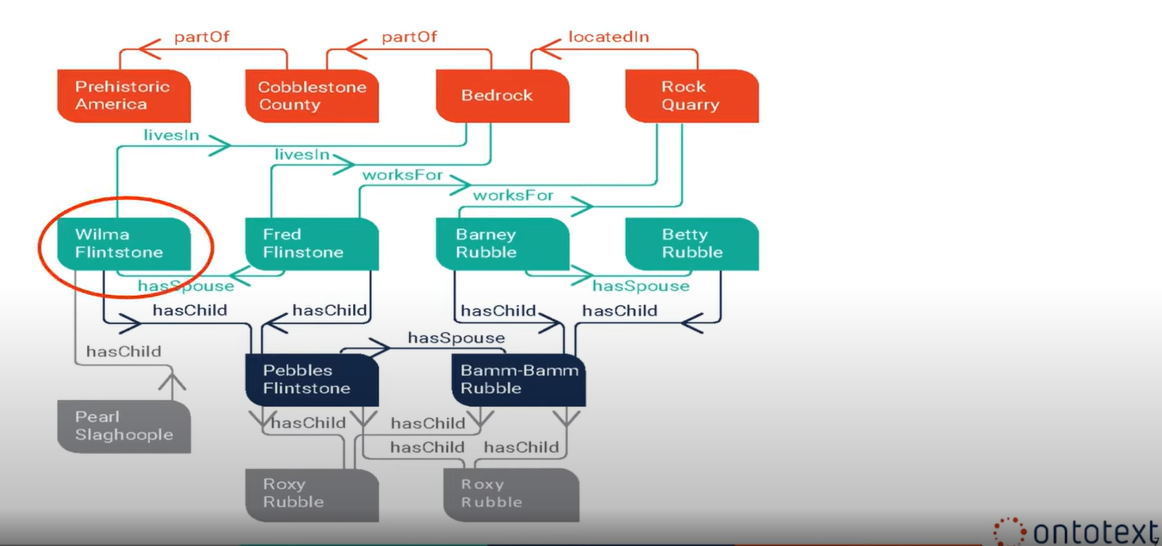
\includegraphics[width=0.8\linewidth,keepaspectratio]{rdf}
\end{center}	  
\end{frame}


%%%%%%%%%%%%%%%%%%%%%%%%%%%%%%%%%%%%%%%%%%%%%%%%%%%%%%%%%%%%%%%%%%%%%%%%%%%%%%%%%%
\begin{frame}[fragile]
\frametitle{Key Features and Applications of RDFS}
\begin{itemize}
\item \textbf{Defining Classes:}
\begin{itemize}
\item RDFS allows us to define classes, representing groups of resources with shared characteristics.
\item Example: In the insurance domain, we can define classes like "Policy," "Customer," and "Claim."
\end{itemize}

\item \textbf{Defining Properties:}
\begin{itemize}
\item RDFS enables us to define properties to describe relationships between resources and classes.
\item Example: We can define properties like "hasCoverage," "belongsTo," and "hasClaim" to link policies, customers, and claims.
\end{itemize}

\item \textbf{Hierarchy and Inheritance:}
\begin{itemize}
\item RDFS supports class hierarchies and inheritance, allowing for more nuanced representations of data.
\item Use Cases: Representing the hierarchical relationship between different types of insurance policies or customer categories.
\end{itemize}

\item \textbf{Use RDFS when}
\begin{itemize}
\item You need a bit more structure in your knowledge graph with the ability to define classes, properties, and hierarchies.
\item Basic inferencing capabilities (e.g., subsumption) are sufficient for your application.
\end{itemize}

\end{itemize}
\end{frame}

%%%%%%%%%%%%%%%%%%%%%%%%%%%%%%%%%%%%%%%%%%%%%%%%%%%%%%%%%%%
\begin{frame}[fragile]\frametitle{RDFS}

\begin{center}
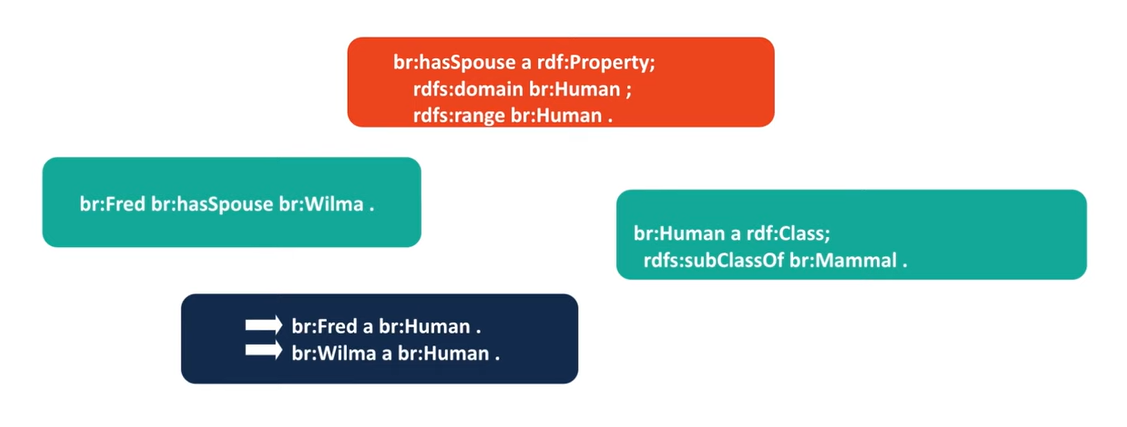
\includegraphics[width=0.8\linewidth,keepaspectratio]{rdfs}
\end{center}	  

hsSpouse relationship is restricted to humans so we can infer that Fred and Wilma are humans and they are mammals.
\end{frame}


%%%%%%%%%%%%%%%%%%%%%%%%%%%%%%%%%%%%%%%%%%%%%%%%%%%%%%%%%%%%%%%%%%%%%%%%%%%%%%%%%%
\begin{frame}[fragile]
\frametitle{Key Features and Applications of OWL}
\begin{itemize}
\item \textbf{Richer Vocabulary:}
\begin{itemize}
\item OWL provides a wide range of constructs for defining classes, properties, and relationships, enabling more precise modeling.
\item Example: Representing intricate insurance policies with multiple coverage options and exclusions.
\end{itemize}

\item \textbf{Advanced Reasoning:}
\begin{itemize}
\item OWL supports automated reasoning and inferencing, allowing for the deduction of implicit information from explicit data.
\item Use Cases: Detecting potential inconsistencies in insurance policies or automatically inferring customer preferences based on their interactions.
\end{itemize}

\item \textbf{Real-World Complexities:}
\begin{itemize}
\item OWL enables the representation of real-world complexities in the insurance domain, such as temporal aspects, uncertainty, and probabilistic relationships.
\item Use Cases: Modeling the dynamic nature of insurance claims processing or incorporating risk probabilities into underwriting decisions.
\end{itemize}

\item \textbf{Use OWL when}
\begin{itemize}
\item Your knowledge graph requires advanced modeling capabilities and complex relationships between entities.
\item You need robust reasoning and inferencing to draw logical conclusions from your data.
\item You want to build ontologies with formal semantics to ensure consistency and reasoning.
\end{itemize}

\end{itemize}
\end{frame}

%%%%%%%%%%%%%%%%%%%%%%%%%%%%%%%%%%%%%%%%%%%%%%%%%%%%%%%%%%%
\begin{frame}[fragile]\frametitle{OWL}

\begin{center}
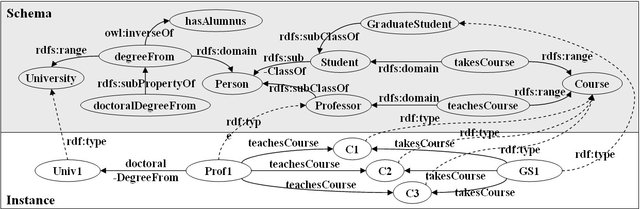
\includegraphics[width=0.8\linewidth,keepaspectratio]{owl}

{\tiny (Ref: An Efficient and Scalable Management of Ontology)}
\end{center}	  

\end{frame}